\chapter{Экспериментальные методы измерения коллективной анизотропии}

\section{Эксперимент HADES}

\subsection{Кинематические области используемые для определения $Q_1$ векторов}

Для анализа использовались события столкновений тяжелых ядер, вершина которых лежала в следующих границах: $\sqrt{x_v^2+y_v^2}<3$~мм и $z_v \in (-60, 0)$~мм.
Для измерения направленного потока использовались траектории заряженных частиц которые были экстраполированы в вершину столкновения.
Траектории которые имели расстояние до восстановленной точки взаимодействия $>10$~мм не использовались в анализе.
Протоны идентифицировались при помощи информации из время-пролетной системы  TOF. 

Оценка плоскости симметрии в работе производилась по асимметрии распределения заряда спектаторов в детекторе FW. 
Для оценки систематической ошибки вызванной непотоковыми корреляциями были введены 2 дополнительных $Q_1$-вектора из треков заряженных частиц.
Векторы $Q_1$ были построены из протонов c поперечным импульсом $p_T < 2.0$~ГэВ с быстротами $0.35 < y_{cm} < 0.55$ (Mf) и $-0.55 < y_{cm} < -0.35$ (Mb).
Модули детектора FW были разделены на 3 группы: центральные (W1), средние (W2) и периферические (W3).
Схематически расположение полученных векторов в плоскости $\eta$-$p_T$ изображено на рис~\ref{fig:hades_qvectors}.
%
\begin{figure}[ht]
\begin{center}
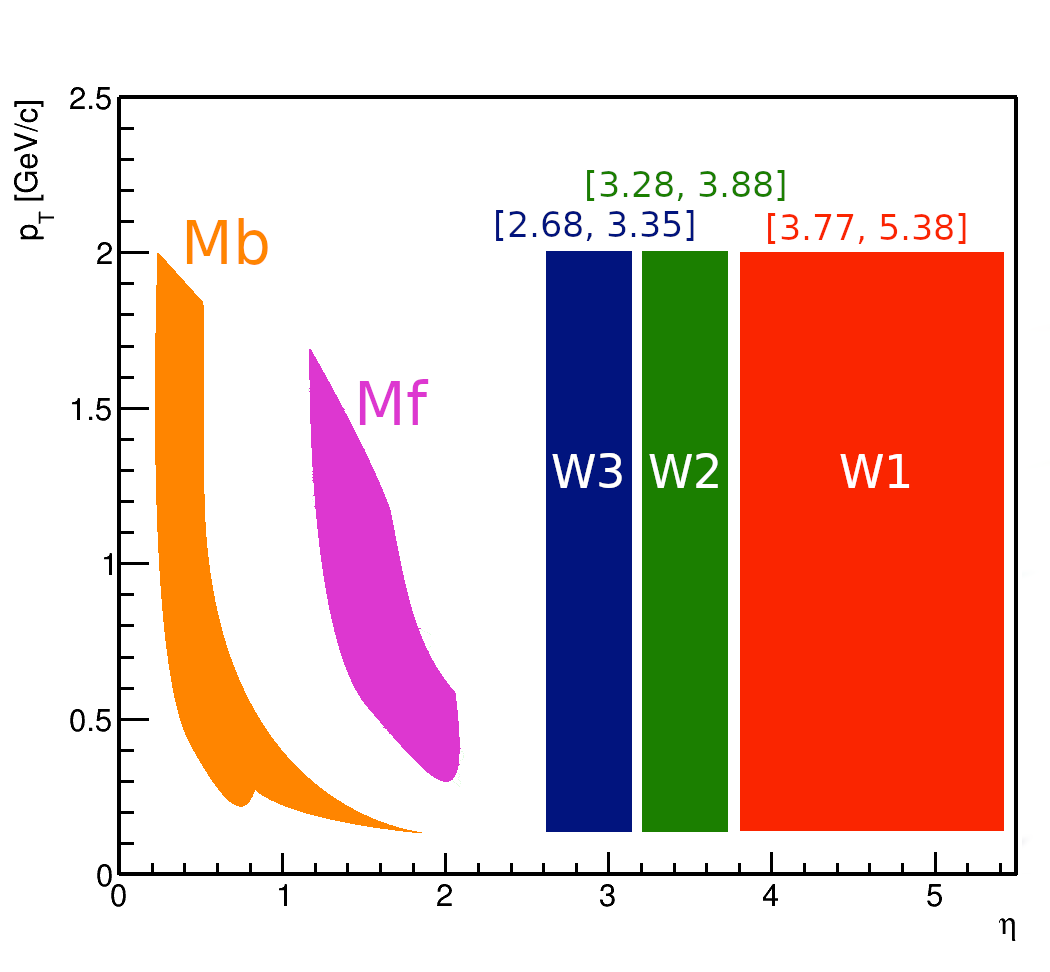
\includegraphics[width=0.75\linewidth]{images/eta_pt_qvectors.png}
\caption{Aксептанс по псевдобыстроте $\eta$ для подсобытий из FW и поперечному импульсу $p_T$ для подсобытий из MDC, использованных для расчета направленного потока протонов в столкновениях ядер золота и серебра.}
\label{fig:hades_qvectors}
\end{center}
\end{figure}
%

\subsection{Коррекция азимутальной анизотропии аксептанса детектора}

Для коррекции на азимутальную неоднородность аксептанса был использован метод, предложенный в~\cite{Selyuzhenkov:2007zi}.
Данный метод основан на предположении, что азимутальное распределение частиц, рожденных в столкновении должно быть изотропным, поскольку угол плоскости реакции от события к событию распределен равномерно.
Азимутальная неоднородность чувствительного объема детектора вносит искажения в азимутальное распределение частиц. 
Для коррекции на этот эффект, в статье~\cite{Selyuzhenkov:2007zi} вводятся поправки перецентровки, поворота и ремасштабирования. 
Схематически, действие этих поправок представлено на рис.~\ref{fig:qn_corrections}.
%
\begin{figure}[ht]
\begin{center}
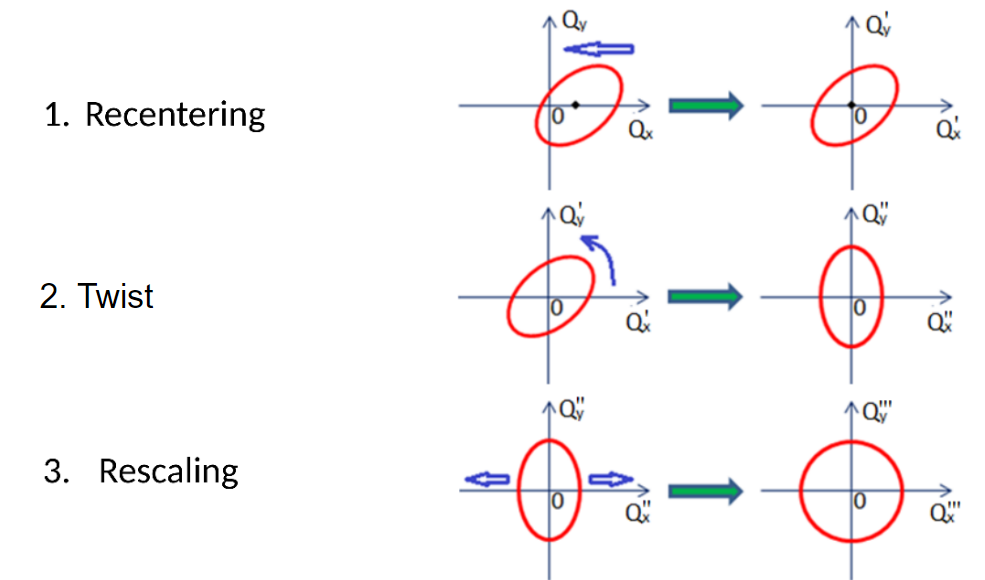
\includegraphics[width=0.75\linewidth]{images/qntools_corrections.png}
\caption{Схематическое изображение поправок предложенных в~\cite{Selyuzhenkov:2007zi}.}
\label{fig:qn_corrections}
\end{center}
\end{figure}
%

Описанные выше поправки применялись для коррекции азимутальной неоднородности аксептанса детектора мультидифференциально.
Для $Q_1$-векторов коррекции применялись в каждом классе центральности от 0\% до 40\% с шагом 5\%.
Для поправок на азимутальную неоднородность трекинга, коррекции на $u_1$-вектор применялись аналогично в каждом классе центральности а также дифференциально по поперечному импульсу $p_T$ и быстроте $y_{cm}$. 
Остаточные эффекты азимутальной неоднородности аксептанса в данной работе оцениваются как разность между корреляцией компонент $u_1$ и $Q_1$-векторов:
\begin{equation}
    \delta_{acc.} = | \langle x_1 X_1 \rangle - \langle y_1 Y_1 \rangle |,
\end{equation}
где $\delta_{acc.}$ --- остаточная ошибка после применения коррекций, $x_1$ и $y_1$, и $X_1$ и $Y_1$ --- компоненты $u_1$ и $Q_1$-векторов соответственно. 

Сравнение $v_1^{uncorr.}$, полученного с использованием различных компонент $u_1$ и $Q_1$-векторов, представлено на рис~\ref{fig:hades_uq_corr}. 
Направленный поток не корректирован на разрешение плоскости симметрии для оценки вклада неоднородного аксептанса трекинговой системы. 
После применения поправок на азимутальную анизотропию аксептанса, остаточный эффект составляет 2\%.
%
\begin{figure}[ht]
\begin{center}
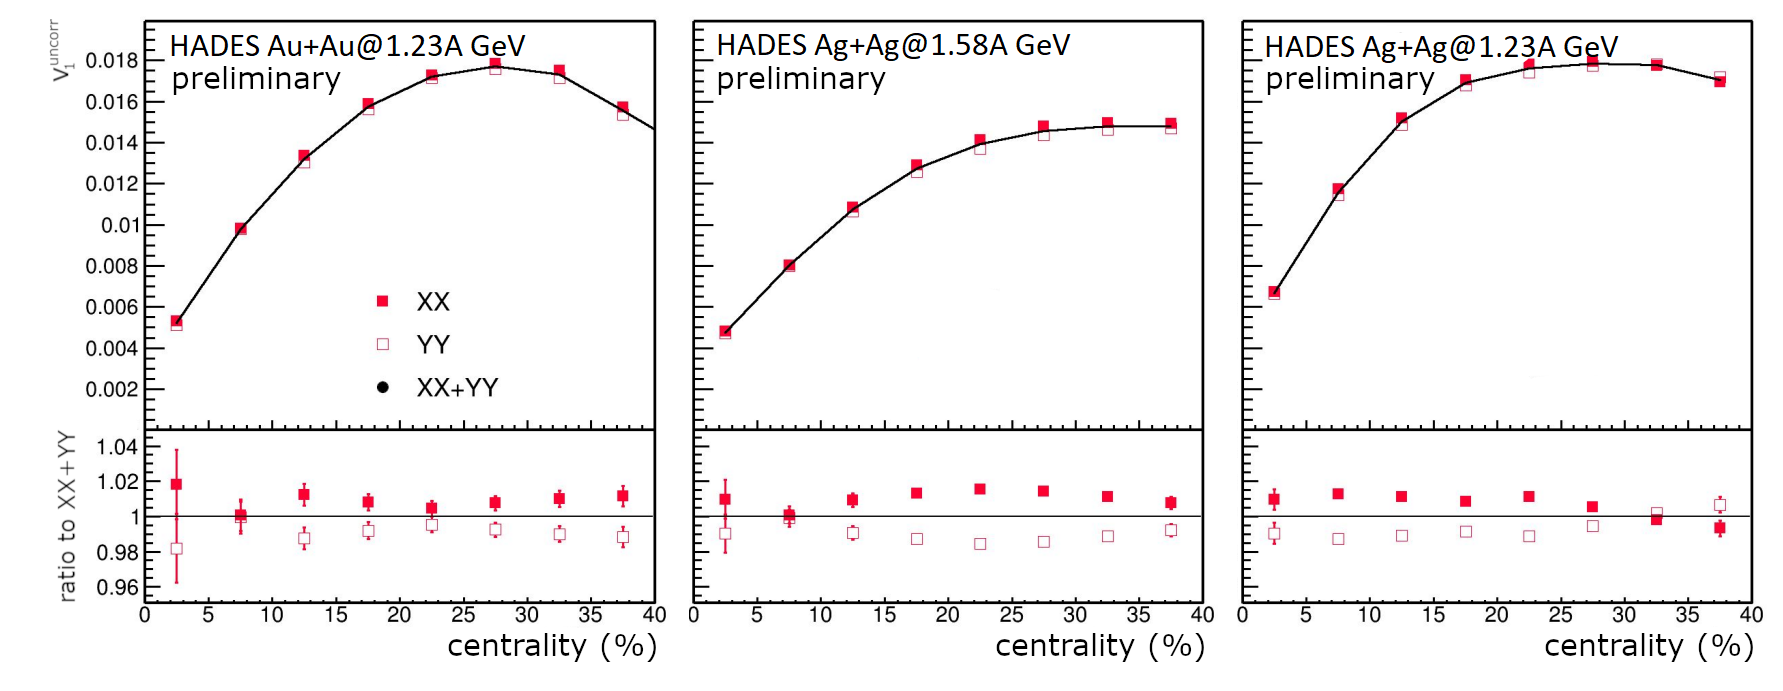
\includegraphics[width=0.75\linewidth]{images/hades_u1W1_centrality.png}
\caption{Сравнение компонент корреляции $\langle u_1 Q_1 \rangle$ после применения поправок на азимутальную неоднородность детектора для столкновений Au+Au@1.23A ГэВ (слева), Ag+Ag@1.23A ГэВ (посередине) и Ag+Ag@1.58A ГэВ (справа)}
\label{fig:hades_uq_corr}
\end{center}
\end{figure}
%

\subsection{Вычисление поравочного коэффициента разрешения $R_1$}

Для рассчета разрешения методом случайных подсобытий два вектора были определены из модулей детектора FW.
Модули были распределены в две группы случайным образом для каждого события.
На рис.~\ref{fig:hades_R1_rs} представлено разрешение плоскости симметрии рассчитанное методом случайных подсобытий как функция центральности столкновения.
Основным недостатком данного метода является отсутствие возможности сравнить полученные значения с другими оценками разрешения плоскости симметрии.
%
\begin{figure}[ht]
\begin{center}
    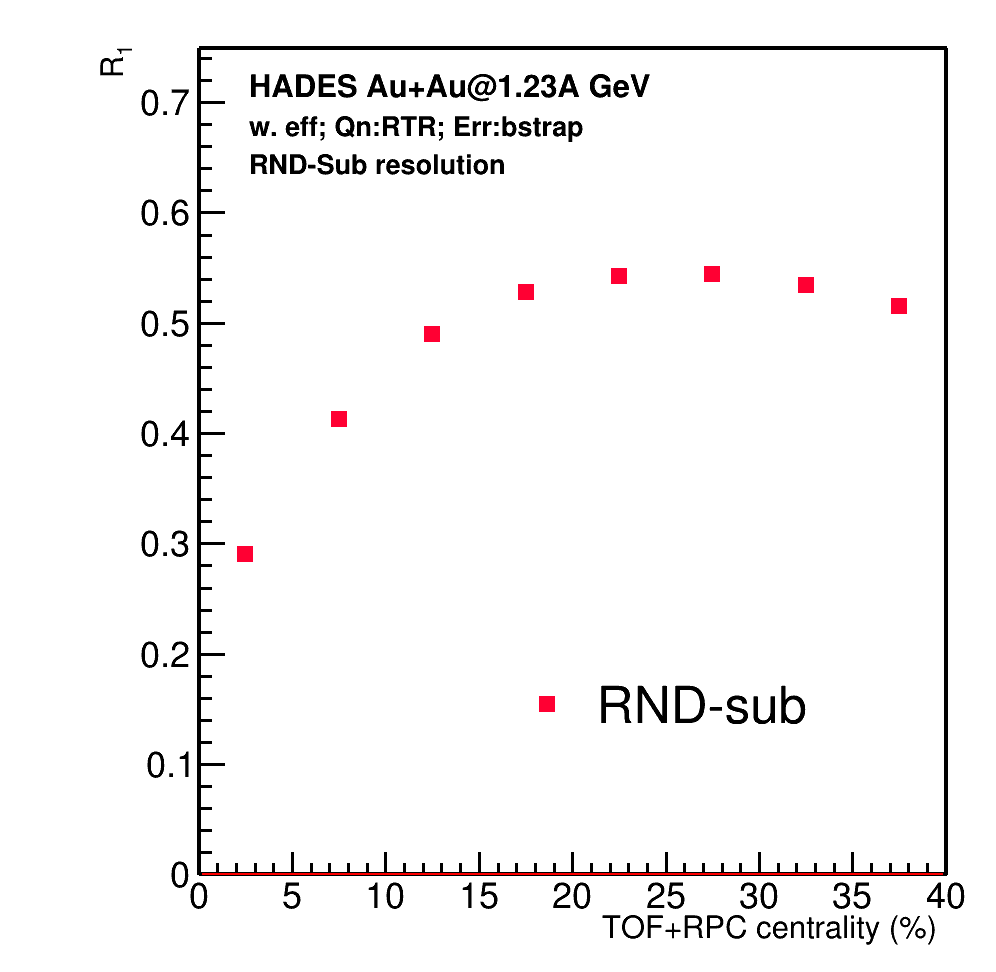
\includegraphics[width=0.3\linewidth]{images/R1_au123_rnd_centrality.png}
    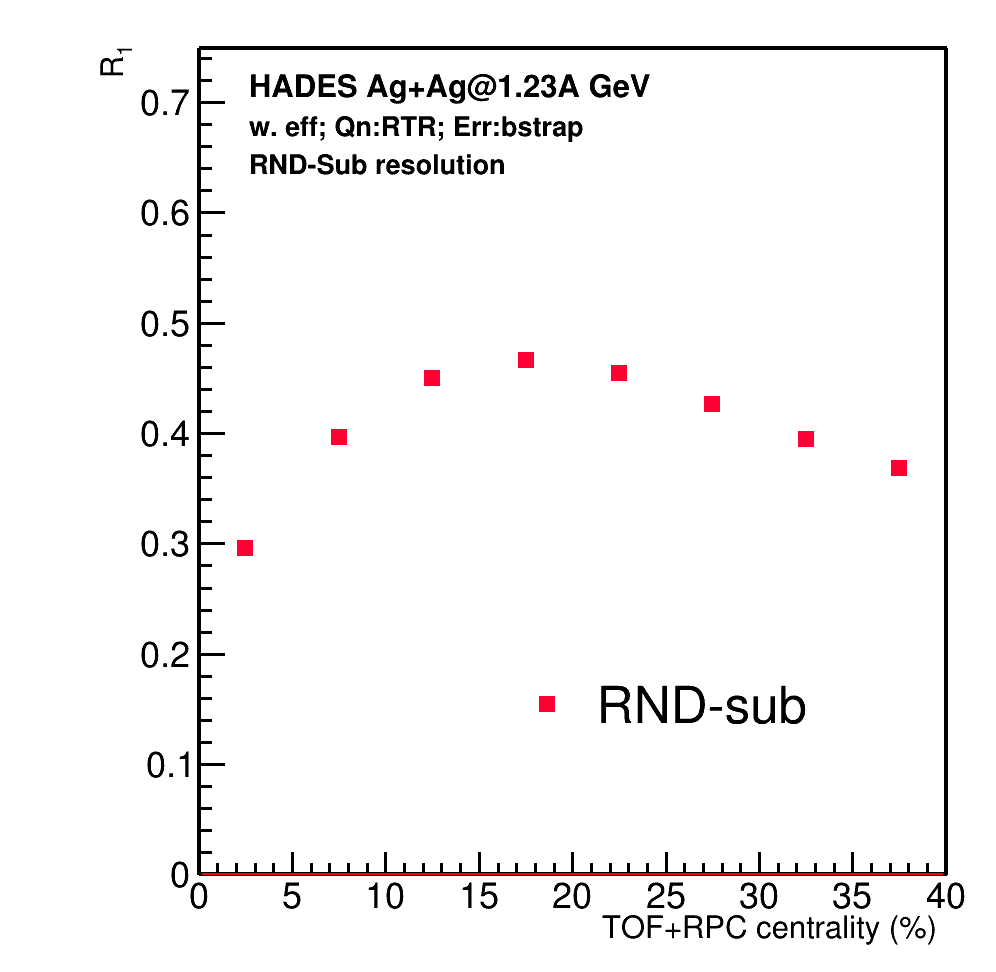
\includegraphics[width=0.3\linewidth]{images/R1_ag123_rnd_centrality.png}
    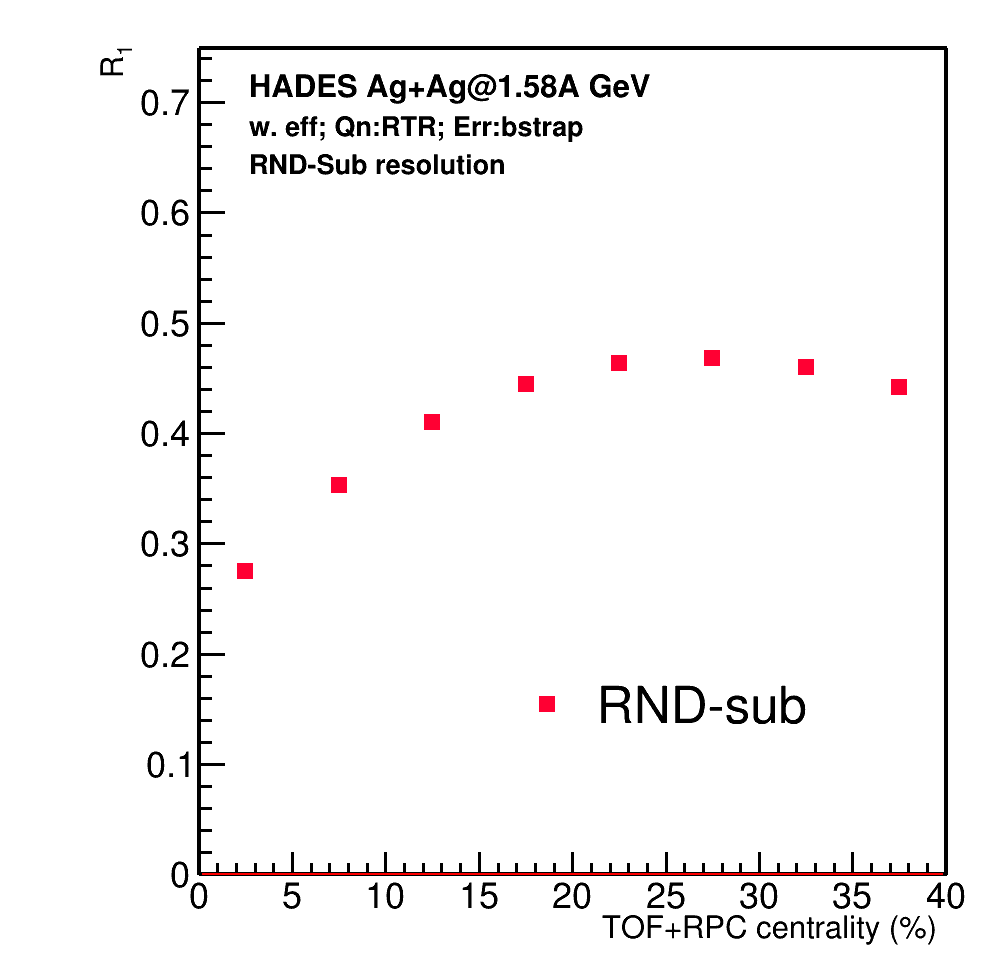
\includegraphics[width=0.3\linewidth]{images/R1_ag158_rnd_centrality.png}
    \caption{Разрешение плоскости симметрии рассчитанное методом случайных подсобытий как функция центральности столкновения.
    Слева: для столкновений Au + Au при $E_{kin}$=1.23$A$~ГэВ;
    посередине: для столкновений Ag + Ag при $E_{kin}$=1.23$A$~ГэВ; 
    справа: для столкновений Ag + Ag при $E_{kin}$=1.58$A$~ГэВ; 
    }
    \label{fig:hades_R1_rs}
\end{center}
\end{figure}
%

Для расчета разрешения методом трёх подсобытий в работе введены 5 $Q_1$-векторов. 
Используя в методе трех подсобытий различные комбинации векторов, можно оценить остаточные эффекты из-за непотоковых корреляций. 
Очевидно, что разрешение плоскости симметрии, посчитанное с использованием различных комбинаций, должны совпадать, а возможная разница будет связана с эффектами не относящимися к коллективному движению частиц.
Исключая из анализа разрешение полученное при помощи комбинаций, в которых два или более векторов коррелируют по непотоковому каналу, можно значительно уменьшить вклад непотоковых корреляций в полученные результаты.
Таким образом, систематическая ошибка из-за эффектов, не связанных с коллективным движением частиц может быть рассчитана следующим образом:
\begin{equation}
    \delta_{NF} = R_1\{a(b,c)\} - R_1\{d(e,f)\},
\end{equation}
где $\delta_{NF}$ --- ошибка из-за непотоковых корреляций, а символами от $a$ до $f$ обозначены различные $Q_1$-вектора.

Разрешение плоскости симметрии $W1$, полученное с использованием различных комбинаций $Q_1$-векторов, показано на рис~\ref{fig:hades_w1_combinations}.
Разрешение $R_1\{W1(W2,W3)\}$ заметно отличается от значений, полученных при помощи других комбинаций. 
Этот эффект может быть объяснён наличием непотоковых корреляций между парами $Q_1$-векторов $W1$ и $W2$, $W2$ и $W3$.
Эти векторы не имеют значительного разделения по быстроте, поэтому в значительной степени могут быть подвержены корреляциям не связанным с изначальной асимметрией области перекрытия. 
В столкновениях Ag+Ag при обеих энергиях, $R_1\{W1(Mf,Mb)\}$ так же значительно отклоняется от среднего результата. 
Это может быть вызвано наличием корреляций из-за закона сохранения импульса между векторами $Mf$ и $Mb$. 
В столкновениях Au+Au этот эффект менее выражен в силу большей множественности рождённых частиц.
%
\begin{figure}[ht]
\begin{center}
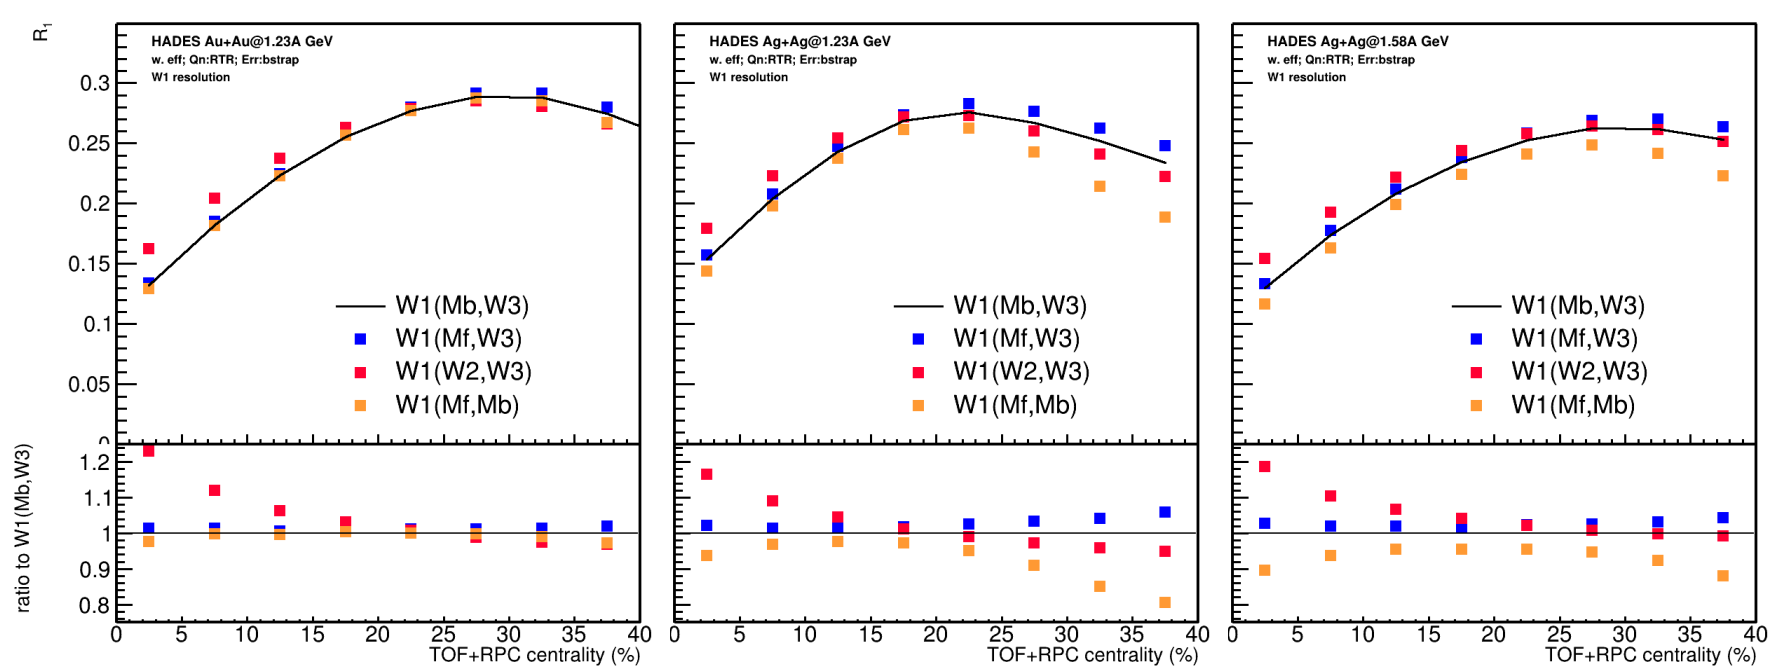
\includegraphics[width=0.75\linewidth]{images/W1_combinations.png}
\caption{Сравнение разрешений плоскости симметрии $W1$ полученное с использованием различных комбинаций $Q_1$-векторов для Au+Au@1.23A ГэВ (слева), Ag+Ag@1.23A ГэВ (посередине) и Ag+Ag@1.58A ГэВ (справа)}
\label{fig:hades_w1_combinations}
\end{center}
\end{figure}

\section{Эксперимент BM@N}

\subsection{Кинематические окна, в которых были определены $Q_1$-вектора}

Для восстановления плоскости симметрии в эксперименте BM@N была использована информация с калориметра FHCal.
Модули детектора были разделены на 3 группы согласно их псевдобыстроте (F1, F2 и F3).
Схематические группы модулей изображены различными цветами на рис.~\ref{fig:bmn_subevents} слева.

Дополнительно для исследования вклада непотоковых корреляций в измеренные значения коллективной анизотропии были введены два $Q_1$-вектора из треков заряженных частиц. 
Вектор $Tp$ построен для протонов со значениями быстроты $0.4<y_{cm}<0.6$ и поперечным импульсом $0.2<p_{T}<2.0$~$GeV/c$.
Вектор $T\pi$ формировался для отрицательных пионов с быстротой и поперечным импульсом $0.2<y_{cm}<0.8$ и $0.1<p_T<0.5 GeV/c$ соответственно.
Соответствующие кинематические области изображены красными прямоугольниками на рис.~\ref{fig:bmn_subevents} справа.
%
\begin{figure}[ht]
\begin{center}
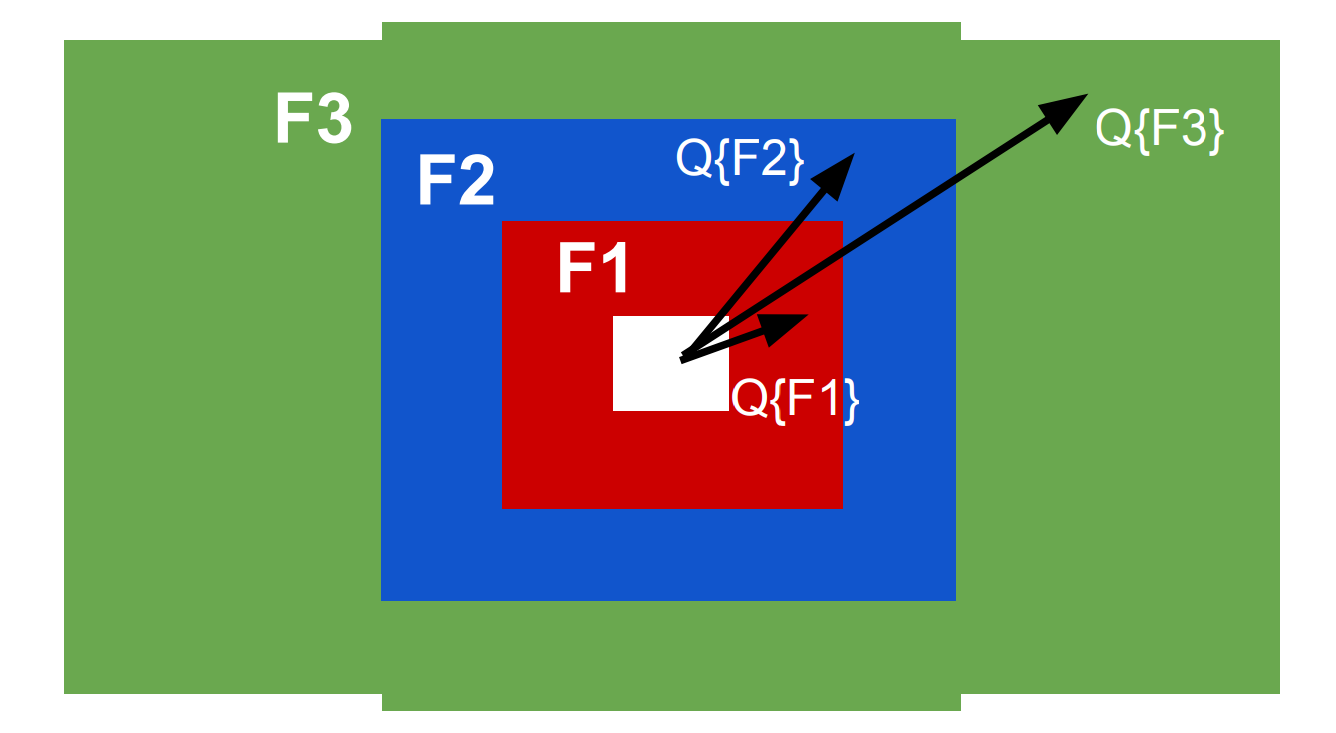
\includegraphics[width=0.45\linewidth]{images/FHCal_layout.png}
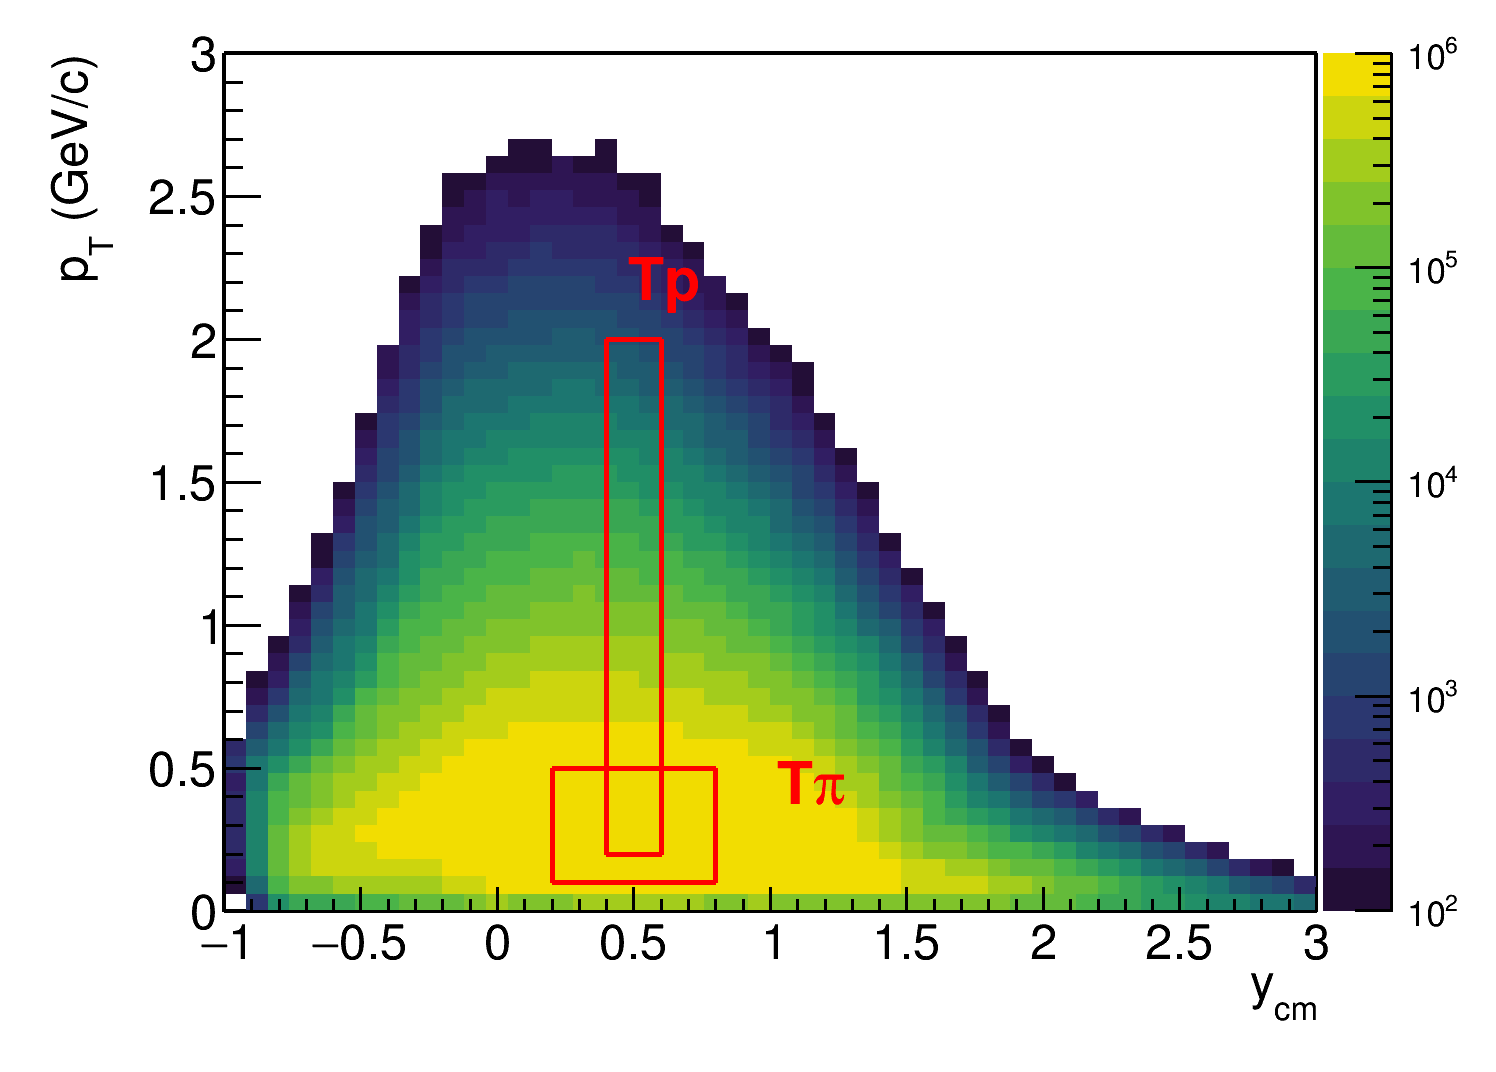
\includegraphics[width=0.45\linewidth]{images/pT_ycm_protons.png}
\caption{
Слева: Схема разделения модулей переднего адронного калориметра по группам для определения плоскости симметрии события.
Справа: Кинематические окна для подсчета $Q_1$-векторов из треков заряженных частиц.
}
\label{fig:bmn_subevents}
\end{center}
\end{figure}

\section{Выводы к главе 3}

В главе обсуждаются методы определения плоскости симметрии столкновения а также способы вычисления разрешения плоскости симметрии при помощи переднего годоскопа FW в эксперименте HADES.
Приводятся результаты применения коррекций на азимутальную анизотропию аксептанса установки HADES и обсуждаются остаточные систематические погрешности, связанные с этим эффектом.
В главе представлены значения поправочного коэффициента разрешения $R_1$ для плоскостей симметрии, определенных при помощи переднего годоскопа FW.
Обсуждаются методы минимизации систематической ошибки связанной с непотоковыми корреляциями и вычисляется остаточная систематическая ошибка.
В главе представлены кинематические диапазоны, использованные для вычисления $Q_1$-векторов в Монте-Карло симуляции эксперимента BM@N.